\documentclass{article}

\usepackage{tikz}
\usetikzlibrary{intersections}
\usetikzlibrary{calc}
\usetikzlibrary {arrows.meta}

\begin{document}

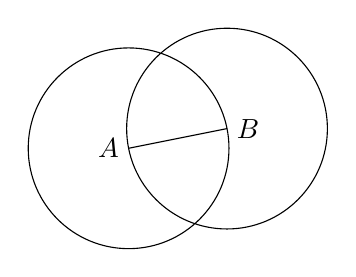
\begin{tikzpicture}
  \coordinate [label=left:$A$]  (A) at (0,0);
  \coordinate [label=right:$B$] (B) at (1.25,0.25);
  \draw (A) -- (B);

  \draw let \p1        = ($ (B) - (A) $),
            \n{radius} = {veclen(\x1,\y1)}
        in
          (A) circle (\n{radius})
          (B) circle (\n{radius});
\end{tikzpicture}

\usetikzlibrary {through}
\begin{tikzpicture}
  \coordinate [label=left:$A$]  (A) at (0,0);
  \coordinate [label=right:$B$] (B) at (1.25,0.25);
  \draw (A) -- (B);

  \node [draw,circle through=(B),label=left:$D$] at (A) {};
\end{tikzpicture}

\usetikzlibrary {intersections,through}
\begin{tikzpicture}
  \coordinate [label=left:$A$]  (A) at (0,0);
  \coordinate [label=right:$B$] (B) at (1.25,0.25);
  \draw (A) -- (B);

  \node (D) [name path=D,draw,circle through=(B),label=left:$D$]  at (A) {};
  \node (E) [name path=E,draw,circle through=(A),label=right:$E$] at (B) {};

  % Name the coordinates, but do not draw anything:
  \path [name intersections={of=D and E}];

  \coordinate [label=above:$C$] (C) at (intersection-1);

  \draw [red] (A) -- (C);
  \draw [red] (B) -- (C);
\end{tikzpicture}

\usetikzlibrary {intersections,through}
\begin{tikzpicture}
  \coordinate [label=left:$A$]  (A) at (0,0);
  \coordinate [label=right:$B$] (B) at (1.25,0.25);
  \draw [name path=A--B] (A) -- (B);

  \node (D) [name path=D,draw,circle through=(B),label=left:$D$]  at (A) {};
  \node (E) [name path=E,draw,circle through=(A),label=right:$E$] at (B) {};

  \path [name intersections={of=D and E, by={[label=above:$C$]C, [label=below:$C'$]C'}}];

  \draw [name path=C--C',red] (C) -- (C');

  \path [name intersections={of=A--B and C--C',by=F}];
  \node [fill=red,inner sep=1pt,label=-45:$F$] at (F) {};
\end{tikzpicture}

\end{document}
